\chapter{Post-transition metal doping of monolayer $WS_2$}

\section{Introduction}

Single layer TMDC materials present a range of unique optical, electrical and mechanical properties and atomic doping can further extend the potential of TMDCs since it has been predicted that a number of properties can be tuned trough compositional variation. Up until now doping has relied on charge transfer induced by changing the environmental conditions such as surface adsorption, metal contacts and dielectric interfaces. This approach has demonstrated to severely limit the device working conditions thus doping trough stable incorporation of non-volatile metal atoms is highly preferred. Achieving controlled doping is a challenge which is aggravated by the fact that established synthesis protocols for these materials are still lacking.

Doping of monolayer $WS_2$ with post-transition metals has not been reported as yet. Doping of $WS_2$ with post-transition metals can lead to chemisorbed intercalated atoms between layers which can be regarded as analogous to deep level impurities. It can lead to an additional energy level near to the top of the valence band or, alternatively, as a modification of the energy band of the host crystal due to the interaction between the intercalate and W or S atoms \cite{Yacobi1979}\cite{Yacobi1979a}. In particular indium may generate an additional energy state at the top of the valence band which leads to a subsequent upward shift of this band \cite{Deshpande2001}. A gradual increase in this shift with increasing number of intercalating atoms would lead to a linear decrease in the energy gap with increasing In content as observed in In-intercalated bulk $WS_2$ \cite{Deshpande2001}. This led to the demonstration of higher conductivity and photocurrent than both pure $WS_2$ films thus proving to be highly photo-active. Unlike their alkali and alkaline earth metal analogues, In-intercalated bulk $WS_2$ compounds were found to be stable against oxidation when exposed to air or chemical due to a fairly strong guest-host bonding which hinders deintercalation processes and preserving a perfect 2H crystalline phase \cite{Deshpande2001}\cite{Rao1981}. Further, In has lower melting and boiling points than B, Al and Ga enabling doping via CVD or MOCVD synthesis of $WS_2$ at low temperatures. These characteristics make Indium a very interesting prospected dopant of $WS_2$ to pave the way towards applications as photoelectrodes in solar cells. Post transition metals are prone to intercalate between the layers however displaying very different effect with respect to the alkali and alkaline earth metal intercalates of $WS_2$.

Here we demonstrate indium doping of monolayer $WS_2$ in–situ during CVD synthesis of $WS_2$. The process relies on the addition of a volatile indium precursor which results in large-area In-doped $WS_2$ atomic layers exhibiting tunable optical properties and a semiconducting-to-metallic transition at high doping levels. We also demonstrate controlled indium content from 0 up to 45\% in $WS_2$ maintaining a 2D morphology and atomically thin nature of the material without sacrificing the lateral extension and scalability of the synthesis process.

\section{Results}

The In doped $WS_2$ samples were grown by following the synthesis route developed for the monolayer $WS_2$ as discussed in Chapter \ref{cha:WS2} \cite{Reale2017}. The synthesis was mostly performed by a fellow PhD student Francesco Reale. The main change was to add $In(OH)_3$ powder as an indium precursor to the same crucible as W precursor. Such mixed powders in a crucible were then placed in the centre of the furnace similarly to the established procedure.

A first indication of the effect of indium in the $WS_2$ is provided by the morphology of the triangular domains. SEM and OM images of $WS_2$ domains grown by using different $In(OH)_3/H_2WO_4$ weight ratios [$In_{0.25}WS_2$, $In_{0.5}WS_2$, $In_{0.75}WS_2$, $In_1WS_2$] are shown in Figure \ref{fig:InOMSEMImages}. While from the optical contrast it is possible to see that the monolayer nature of the domains is unchanged, it can be noticed how the shape of triangles progressively change. Triangles with straight edges similar to that of pristine $WS_2$ are displayed for low In content while convex and jagged edges appear by increasing the Indium content, which might suggest a more significant incorporation of the latter. $WS_2$ with high indium content can also present different morphologies and even large coverage.

\begin{figure}[!ht]
	\begin{center}
		\begin{subfigure}[b]{0.7\textwidth}
			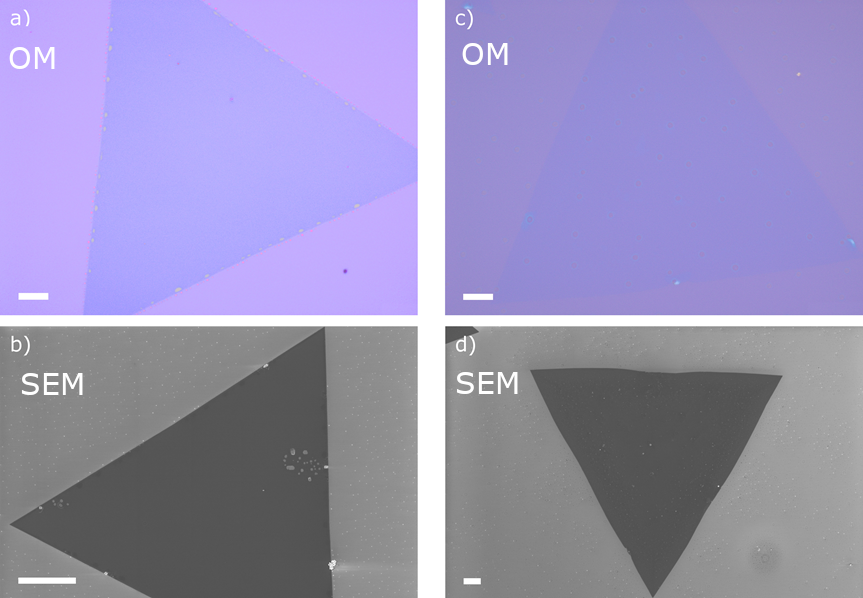
\includegraphics[width=\textwidth]{In/OMSEMImages1.png}
			\label{fig:InOMSEMImages1}
		\end{subfigure}
		\qquad
		\begin{subfigure}[b]{0.7\textwidth}
			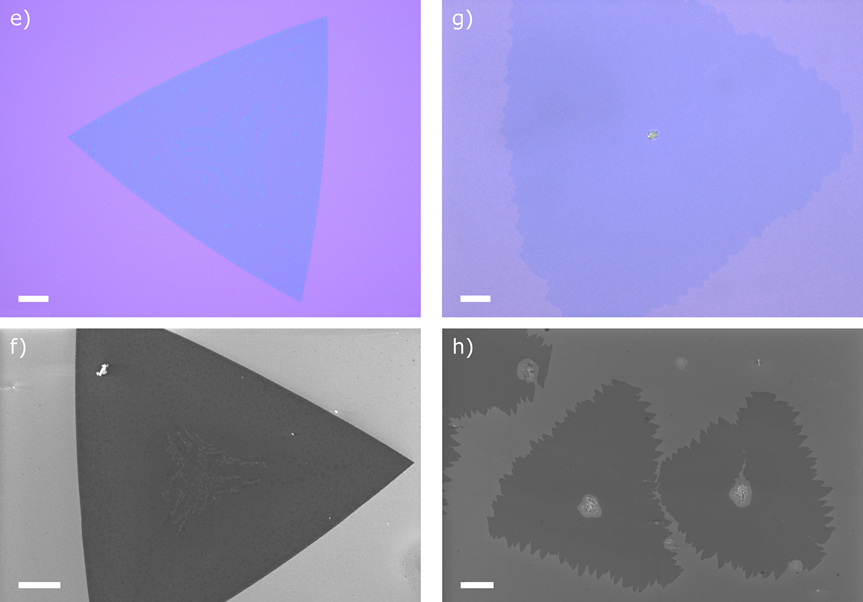
\includegraphics[width=\textwidth]{In/OMSEMImages2.png}
			\label{fig:InOMSEMImages2}
		\end{subfigure}
		\caption{OM and SEM images of flakes grown with different $In(OH)_3/H_2WO_4$ weight ratios: (a, b) 0.25, (c, d) 0.5, (e, f) 0.75 and (g, h)=1. Scale bar is 10 $\mu m$}
		\label{fig:InOMSEMImages}
	\end{center}
\end{figure}

The samples were further characterised using XPS to assess the exact chemical content and therefore the level of doping.

\begin{figure}[H]
	\begin{center}
		\begin{subfigure}[b]{0.6\textwidth}
			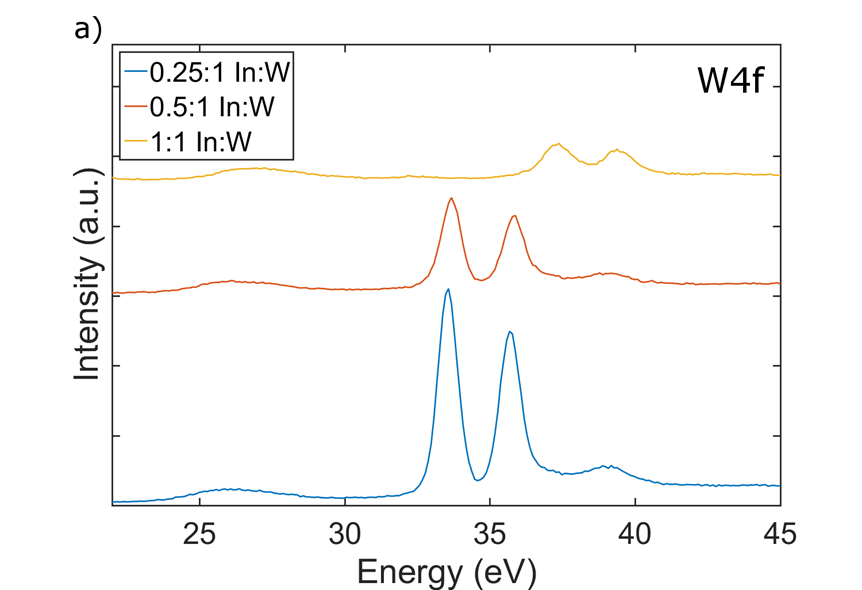
\includegraphics[width=\textwidth]{In/XPSW4f.png}
			\caption{W 4f}
			\label{fig:InXPSW4f}
		\end{subfigure}
		\qquad
		\begin{subfigure}[b]{0.6\textwidth}
			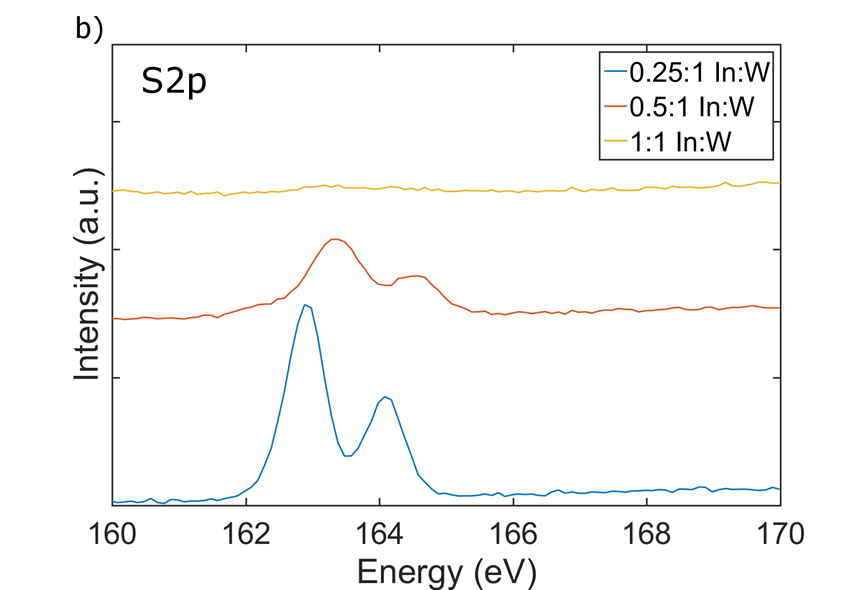
\includegraphics[width=\textwidth]{In/XPSS2p.png}
			\caption{S 2p}
			\label{fig:InXPSS2p}
		\end{subfigure}
		\begin{subfigure}[b]{0.6\textwidth}
			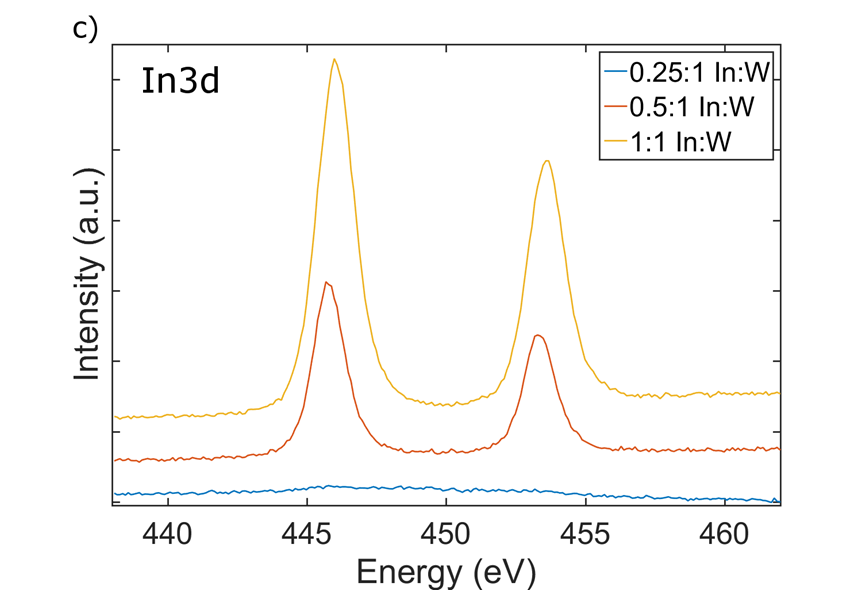
\includegraphics[width=\textwidth]{In/XPSIn3d.png}
			\caption{In 3d}
			\label{fig:InXPSIn3d}
		\end{subfigure}
		\caption{XPS spectra comparison}
		\label{fig:InXPSSpectra}
	\end{center}
\end{figure}

Figure \ref{fig:InXPSSpectra} shows the In 3d, W 4f and S 2p core levels XPS spectra for pure $WS_2$ and In-doped $WS_2$ (In/W=0.25, In/W=0.5, In/W=1). It is immediately noticable in Figure \ref{fig:InXPSIn3d} that the the sample with 0.25:1 In:W precursor ratio does not exhibit any In 3d peak. At the same time the samples with 0.5:1 In:W as well as 1:1 In:W show pronounced In $3d_{5/2}$ core level peak at 445.8 eV and 446.0 eV respectively and In $3d_{3/2}$ at 453.3 eV and 453.8 eV respectively. This slight shift might be attributed to the presence of $In_xW_yS_z$ compounds \cite{Wagner1991}. The In 3d core levels for 1:1 In:W sample are also about twice as intense as the ones for the 0.5:1 In:W sample. Furthermore the W 4f core levels for the 1:1 In:W sample are significantly shifted to the blue which might indicate presence of $W^{6+}$ in the doped sample compared to $W^{4+}$ to pure $WS_2$. This would indicate bonding between W and In atoms. The S $2p_{1/2}$ and S $2p_{3/2}$ core levels for 0.25:1 In:W ratio can be observed at 162.9 eV and 164.1 eV respectively while for the 0.5:1 In:W sample they are at 163.4 eV and 164.6 eV respectively. No significant S 2p peak can be observed for the 1:1 In:W ratio sample. There is therefore indication of interaction between the S and In atoms, with stronger S 2p core level peak shifts than those of the W 4f core levels. It is therefore possible that the In atoms became chemisorped on the surface, intercalated in between the layers or incorporated as an interstitial. The stoichiometric composition was then calculated using the concentrations of elements from peak integration of In 3d, W 4f and S 2p core levels as seen in Table \ref{tab:InRatios}.

\begin{table}[!ht]
\caption{In:W and S:W ratios obtained by calculating the In, W and S concentrations from the integrated intensity of the In 3d, W 4f and S 2p core levels.}
\label{tab:InRatios}
\end{table}

\begin{center}
\begin{tabular}{c|cc}

Sample 		& In/W 		& S/W\\\hline
In/W = 0.25 & 0.038:1 	& 2.32:1\\
In/W = 0.5	& 0.45:1	& 2.22:1\\
In/W = 1	& 1.98:1	& 0.27:1

\end{tabular}
\end{center}

The XRD diffraction patterns of all the In-doped $WS_2$ samples can all be indexed on a hexagonal unit cell basis (Figure \ref{fig:InXRDAll}) and an analogy can drawn to the pattern of $2H-WS_2$. The set of reflections can be then used to calculate the lattice parameters in a known crystal structure. The most intense reflection is the (002) and for pure and In-doped $WS_2$ (Figure \ref{fig:InXRDIn}) it can be seen that the FWHM decreases as the In precursor concentration increases and that a peak shift towards a larger d spacing, the height of single layer, (Table \ref{tab:InXRDData}) occurs for the highest indium content. Additionally the samples with indium content of In/W=0.5, In/W=0.75 and In/W=1 show an additional reflection at $2{\Theta}=13.44$ not belonging to $WS_2$, which can be an indicator of successful incorporation of In atoms.

\begin{table}[!ht]
\caption{Data for the (002) XRD peak and lattice parameters for pure $WS_2$ and In-doped $WS_2$ samples.}
\label{tab:InXRDData}
\end{table}

\begin{center}
\begin{tabular}{c|ccccc}

Sample 		& Position (2$\Theta$)	& FWHM (2$\Theta$)	& a (\r{A})	& c (\r{A})	& d (\r{A})	\\\hline
$WS_2$	 	& 14.44 				& 0.703				& 3.23		& 11.02		& 5.51		\\
In/W = 0.25	& 14.47					& 0.294				& 3.23		& 11		& 5.50		\\
In/W = 0.5	& 14.444				& 0.168				& 3.22		& 11.02		& 5.51		\\
In/W = 0.75	& 14.479				& 0.137				& 3.22		& 11		& 5.50		\\
In/W = 1	& 14.307				& 0.182				& 3.21		& 11.14		& 5.57

\end{tabular}
\end{center}

Therefore, it can be concluded that the crystal structure remains unchanged for Indium content of less than 0.038, corresponding to a precursor ratio of In/W = 0.25 as seen in Table \ref{tab:InRatios}. For large indium contents an expansion of the van der Waals gap is observed due to the large amount of indium intercalated between the layers in few-layered regions and also a small portion of indium can result incorporated in the crystal structure. 

From XRD results we can see that the crystal structure remained hexagonal with small shifts in lattice paramters as the indium content increased in the sample. Our results are therefore comparable to previous reports on the In intercalation in bulk $MoS_2$ which showed that smaller ions can lead to a significant change in the crystallographic order \cite{Somoano1979} changing it to a octahedral coordination. It has also been shown that inclusion of the large metal ions (In, Ga) preserves the hexagonal structure \cite{Somoano1979}. The presence of d-bands in indium metal contributes additionally to the bonding stabilization.

\begin{figure}[!h]
	\begin{center}
		\begin{subfigure}[b]{0.7\textwidth}
			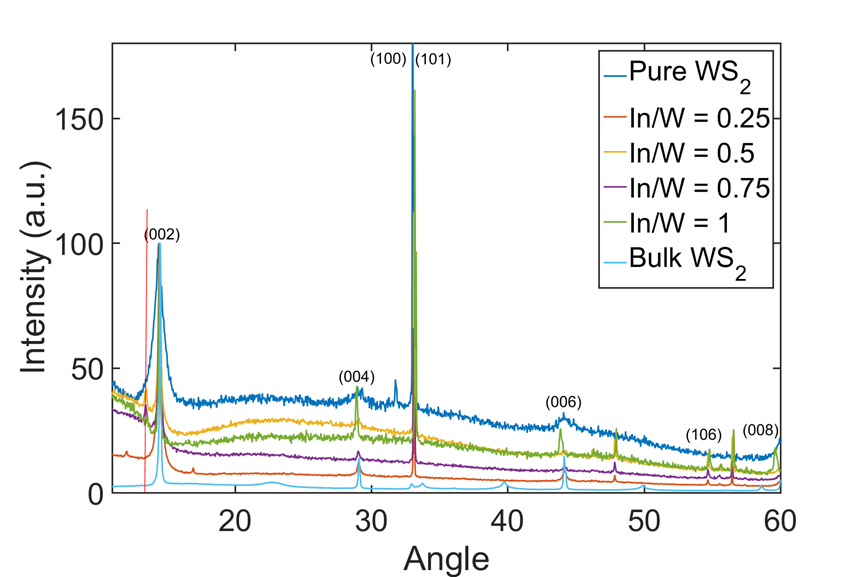
\includegraphics[width=\textwidth]{In/XRDAll.png}
			\caption{XRD patterns for CVD-grown pure $WS_2$ and In-doped $WS_2$.}
			\label{fig:InXRDAll}
		\end{subfigure}
		\qquad
		\begin{subfigure}[b]{0.7\textwidth}
			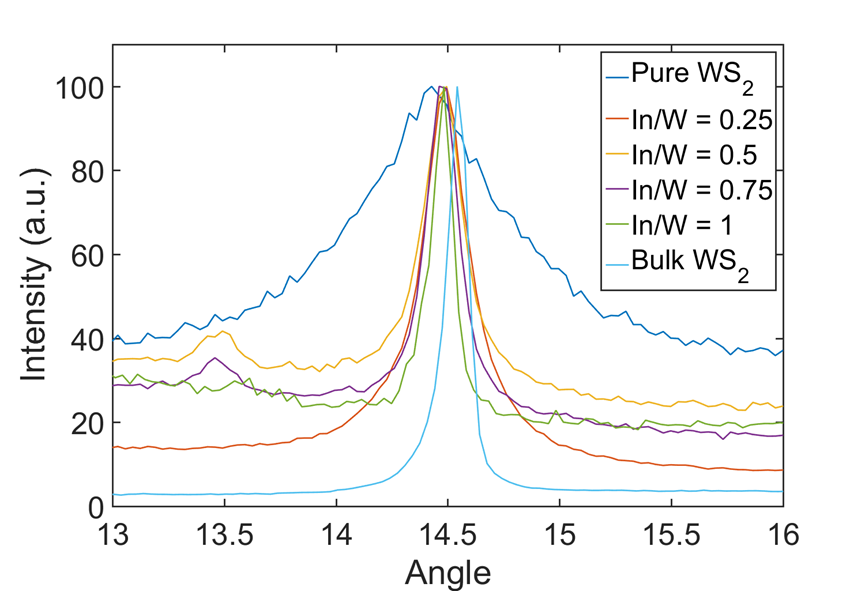
\includegraphics[width=\textwidth]{In/XRDIn.png}
			\caption{(002) XRD peak for CVD-grown pure $WS_2$ and In-doped $WS_2$}
			\label{fig:InXRDIn}
		\end{subfigure}
		\caption{XRD spectra of $WS_2$ samples}
		\label{fig:InXRDSpectra}
	\end{center}
\end{figure}

\begin{figure}[H]
	\begin{center}
		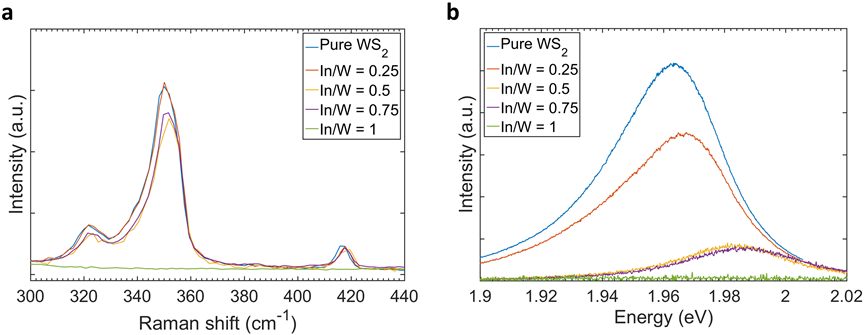
\includegraphics[scale=0.5]{In/RamanPL.png}
		\caption{Representative a) Raman and b) PL spectra for pure $WS_2$ (grown by using $H_2WO_4$ as metal precursor) and In-doped $WS_2$}
		\label{fig:InRamanPL}
	\end{center}
\end{figure}

Further evidence of $In_2S_3$ can be inferred by the presence of peaks at $2\Theta ={\sim}48$ and $\sim$57 \cite{Hahn1949}, specifically the (002) plane. This has been observed in the form of thick crystals in the centre of atomically thin flakes (Figure \ref{fig:InSEMCentre}) and has been confirmed by Raman (Figure \ref{fig:InSEMCentre}). The $In_2S_3$ have been rarely observed and can therefore be the result of secondary reaction products.

\begin{figure}[!h]
	\begin{center}
		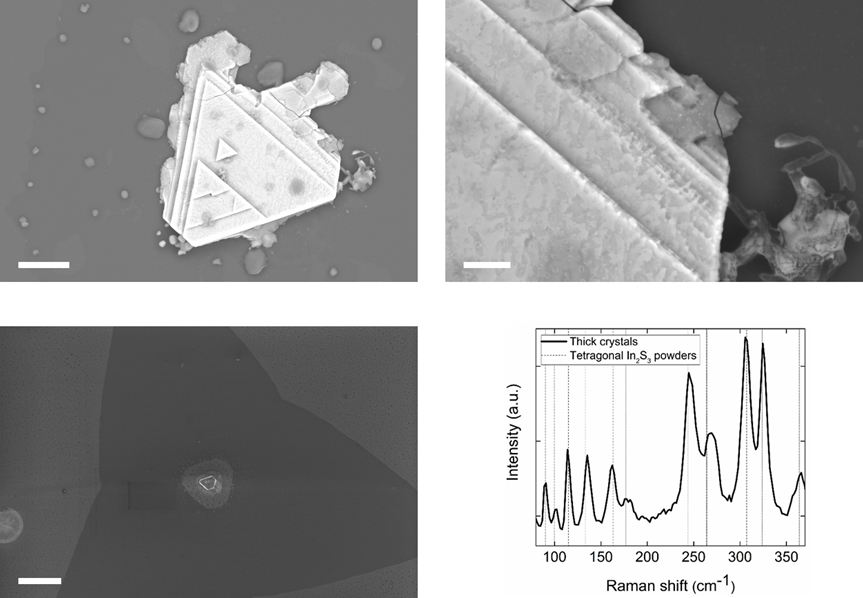
\includegraphics[scale=0.5]{In/SEMCentre.png}
		\caption{Low-magnification SEM images in (a) SE and (scalebar = 2 $\mu m$) (b) BSD imaging mode of the same area of sample In/W=1 (scalebar = 10 $\mu m$). High-magnification SEM images in (c) SE (scalebar = 200 $nm$) and (d) Raman spectrum of the thick flake in a) and c) showing that it consists of $In_2S_3$}
		\label{fig:InSEMCentre}
	\end{center}
\end{figure}

The representative Raman spectra for undoped $WS_2$ and In-doped $WS_2$ are reported in Figure \ref{fig:InRamanPL} a). It can be observed that $WS_2$ sample with In:W ratio of 0.25:1, 0.5:1 and 0.75:1 show the characteristic in-plane $2LA-E^1_{2g}$ and out-of-plane $A_{1g}$ vibrational Raman active modes of $WS_2$, while the sample with In content of 1 is not Raman active. Similarly, $WS_2$ with In content between 0.038-0.45 exhibit PL while $WS_2$ with In content of 1 does not luminescence (Figure \ref{fig:InRamanPL} b)). Therefore, a very large amount of In (equal to 1) changes the crystal lattice and properties of the base material. The $E^1_{2g}$ and $A_{1g}$ Raman peaks (Figure \ref{fig:InRamanPLHistogram}) of the 0.25:1, 0.5:1 and 0.75:1 In-doped samples are shifted towards higher frequencies ($E^1_{2g}$ at $\sim 351.5 cm^{-1}$ and $A_{1g}$ at $\sim 418 cm^{-1}$) as compared to pure $WS_2$ sample. This could be due to the differences in the binding energy between W–S and (W-In)–S bonds. The shifts in Raman peak position observed in mono and few layer thick TMDCs are however not fully yet understood and further characterisations are necessary. 

The excitons-to-trions ratio (Figure \ref{fig:InPLRatioHistogram}) calculated for the samples that exhibit PL is lower compared to that of the undoped $WS_2$, which indicates increase in n doping behaviour as the In content increases. It can be explained due to the presence of fully filled d-orbital in In atoms with an additional electron in the p-orbital in the most outer shell. These extra electrons may therefore contribute to the semiconductor to metal transition with high enough In concentration. To confirm that electrical measurements were performed. Metal contacts were patterned onto one of the flakes on the In:W=1 ratio samples. Conductivity has been measured across the flake and a direct increase in resistivity with increase in temperature has been revealed which is indicative of the metals (Figure \ref{fig:InElectricalMeasurement}).

\begin{figure}[!h]
	\begin{center}
		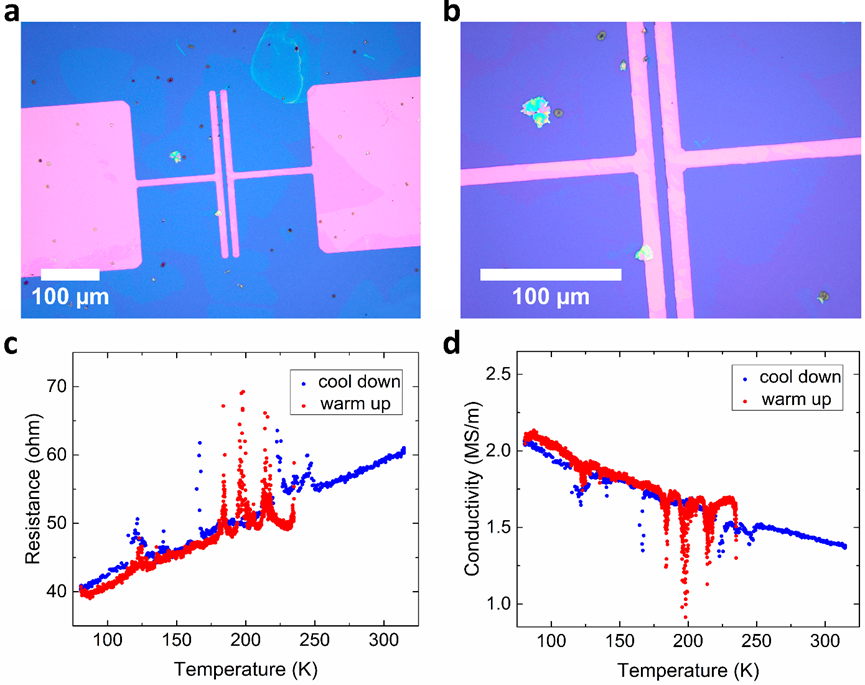
\includegraphics[scale=0.4]{In/ElectricalMeasurements.png}
		\caption{(a, b) Optical micrographs of Ti and Au contacts deposited on In/W=1 flakes. (c) Measured resistance as a function of temperature. (d) Calculated conductivity vs. temperature revealing a semi-metallic behaviour.}
		\label{fig:InElectricalMeasurement}
	\end{center}
\end{figure}

\newpage
\begin{figure}[!h]
	\begin{center}
		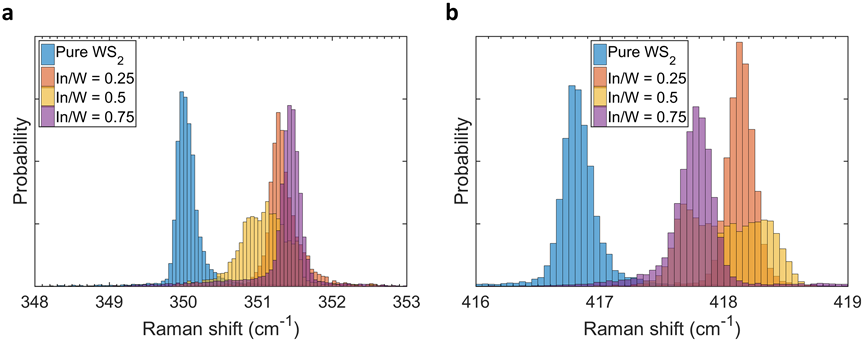
\includegraphics[scale=0.5]{In/RamanPositionHistogram.png}
		\caption{a) $E^1_{2g}$ and b) $A_{1g}$ peak positions for pure $WS_2$ and Raman active In-doped $WS_2$ samples.}
		\label{fig:InRamanPLHistogram}
	\end{center}
\end{figure}

\begin{figure}[H]
	\begin{center}
	\begin{subfigure}[b]{0.55\textwidth}
		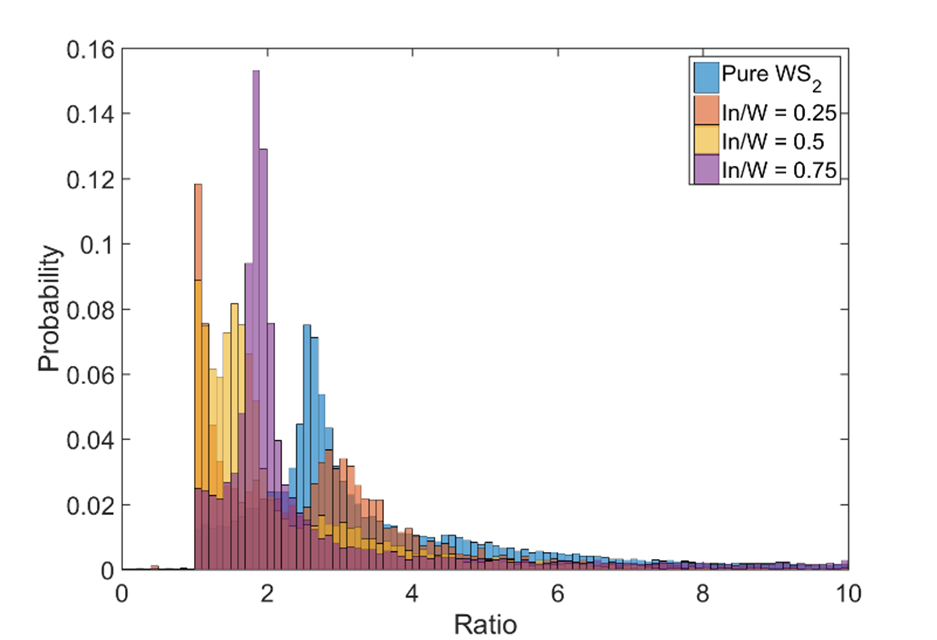
\includegraphics[width=\textwidth]{In/PLRatioHistogram.png}
		\caption{Excitons-to-trions ratio for pure $WS_2$ and PL active In-doped $WS_2$ samples XPS}
		\label{fig:InPLRatioHistogram}
	\end{subfigure}
	\qquad
	\begin{subfigure}[b]{0.55\textwidth}
		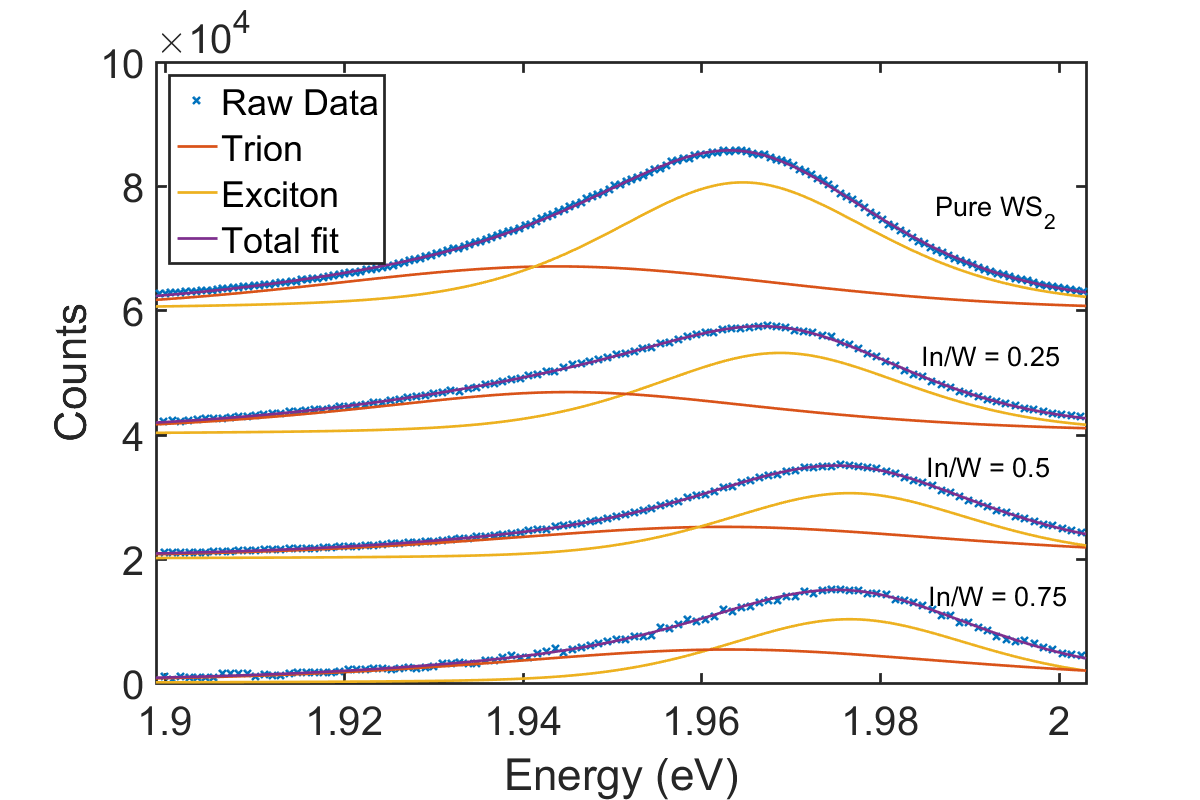
\includegraphics[width=\textwidth]{In/allplotsfitted.png}
		\caption{PL spectra from samples of different In/W precursor ratio.}
		\label{fig:InPLRatioPlots}
	\end{subfigure}
	\end{center}
\end{figure}

The energy dispersive x-ray spectroscopy (EDS) has been then utilised to find the chemical makeup of the sample. First the as grown sample was characterised using SEM EDS which requires no sample transfer. As seen in Figure \ref{fig:InTEMEDSFra} there are In peaks present at: $L_{{\alpha}1} = 3286.94 eV; L_{{\alpha}2} = 3279.29 eV; L_{{\beta}1} = 3487.21 eV; L_{{\beta}2} = 3713.81 eV; L_{{\gamma}1} = 3920.81 eV$. This indicates and further confirms in addition to the XPS results that there is some In in, on or around the $WS_2$ flake. There is also a visible $Na$ peak which indicates remaining $Na$ from $NaCl$ used during synthesis. In order to compare the as grown sample, the transferred sample was characterised using TEM EDS. As seen in Figure \ref{fig:InTEMEDS} there is no visible In peak. This indicates that the In is somehow removed during the transfer process. It is therefore most likely that the In is not present inside the $WS_2$ as a dopant, as substitution or an interstitial, or that it is located in between the layers, but that it is present on top of or around the as grown $WS_2$ flake.

\begin{figure}[H]
	\begin{center}
			\begin{subfigure}[b]{0.6\textwidth}
			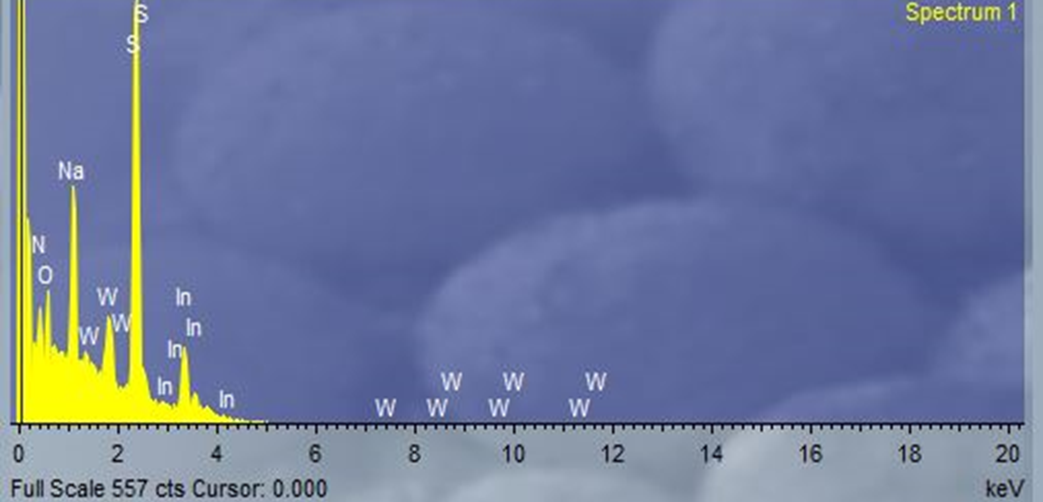
\includegraphics[width=\textwidth]{In/TEMEDSFra.png}
			\caption{Before transfer}
			\label{fig:InTEMEDSFra}
		\end{subfigure}
		\qquad
		\begin{subfigure}[b]{0.6\textwidth}
			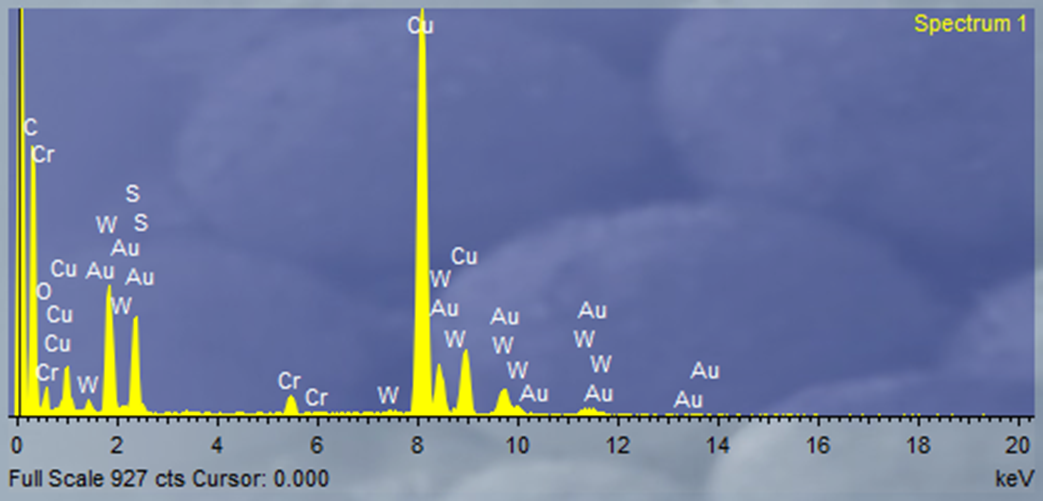
\includegraphics[width=\textwidth]{In/TEMEDS.png}
			\caption{After transfer}
			\label{fig:InTEMEDS}
		\end{subfigure}
		\caption{EDS spectra collected using TEM from $WS_2$ sample with $In:W = 1:2$}
		\label{fig:InTEMEDSSpectra}
	\end{center}
\end{figure}

Additionally the electron diffraction (ED) measurement was performed. As seen in Figure \ref{fig:InTEMED} the present pattern correspond to the expected pattern for $WS_2$. The spots are sharp and narrow indicating mostly monolayer $WS_2$ with no elongation or broadening expected due to the presence of irregular presence of doping element. There is also no additional pattern that could indicate a super structure of ordered atoms of the dopant. The faint halo indicates presence of the amorphous carbon of the TEM grid. The faint signal is therefore indicative of a lack of polymer remains after the transfer. Finally the calculated lattice parameter $a$ was found to be a = 2.71 \r{A} which is in agreement to the $a$ parameter found for the un doped $WS_2$ from the XRD spectrum as seen in Figure \ref{fig:InXRDSpectra} (a = 2.71 \r{A}) as well as the  one found for the bulk $WS_2$ (a = 2.73 \r{A}). This indicates therefore that the transferred sample shows no change in strain after the transfer.

\begin{figure}[H]
	\begin{center}
		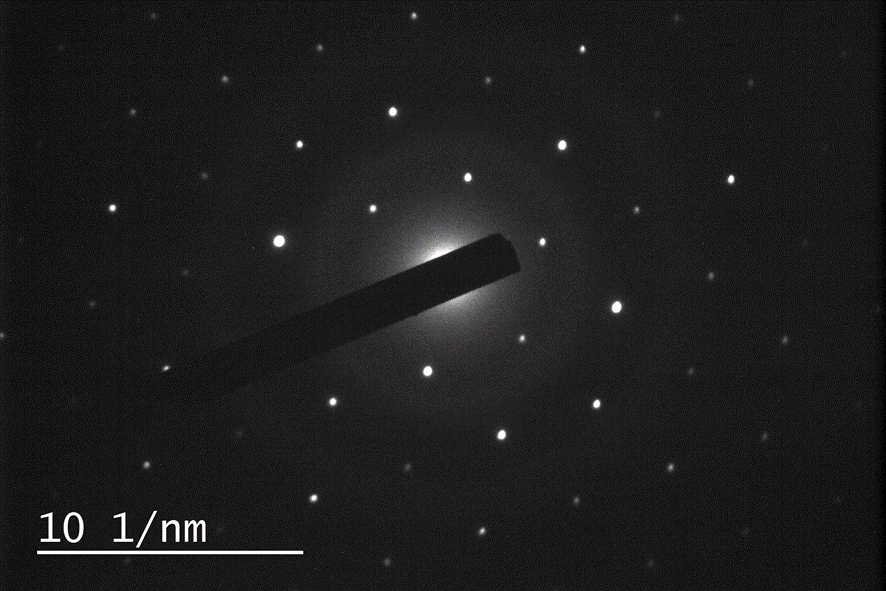
\includegraphics[scale=0.4]{In/TEMED.png}
		\caption{Electron diffraction pattern of $WS_2$ flake with $In:W = 1:2$}
		\label{fig:InTEMED}
	\end{center}
\end{figure}

\section{Conclusions}

In summary, we have reported indium atoms doping of $WS_2$ atomic layers in situ during synthesis, without sacrificing the lateral extension or the reproducibility of the synthesis process. Remarkably, the In-doped $WS_2$ samples exhibit tunable light emission and a semiconducting-to-semimetallic transition at high doping levels. It remains unclear where the In atoms are located after the growth and to what degree are they incorporated into the base material. Moreover the range of In/W ratios from 0.25 to 0.5 needs especially further investigation as it shows a substantial change in In content in the as grown material. Therefore, the present synthesis strategy can be employed to achieve tailorable optical and electrical characteristics of atomically-thin $WS_2$ through stable incorporation of non-volatile post-transition metal atoms.